\documentclass{article}
\usepackage[margin=1in]{geometry}
\usepackage{enumitem}
\usepackage{setspace}
\usepackage{amsmath}
\usepackage{amssymb}
\usepackage{physics}
\usepackage{relsize}
\usepackage{graphicx}

\title{Math 132 Homework 5}
\date{11/3/2020}
\author{Jiaping Zeng}

\begin{document}
\setstretch{1.5}
\maketitle

\begin{itemize}
    \item [3.4.13] $\mathlarger{\int_{C_1(0)}\dfrac{e^z}{z+2}dz}$\\
          \textbf{Answer}: Since the discontinuity $z=-2$ is outside of $C_1(0)$, our function $f(z)=\dfrac{e^z}{z+2}$ is analytic on and inside $C_1(0)$. Therefore we have $\mathlarger{\int_{C_1(0)}\frac{e^z}{z+2}dz}=0$ by Cauchy's integral theorem.
    \item [3.4.15] $\mathlarger{\int_{C_1(i)}\left(\frac{z-1}{z+1}\right)^2zdz}$\\
          \textbf{Answer}: Since the discontinuity $z=-1$ is outside of $C_1(i)$, our function $f(z)=\left(\dfrac{z-1}{z+1}\right)^2$ is analytic on and inside $C_1(i)$. Therefore we have $\mathlarger{\int_{C_1(i)}\left(\frac{z-1}{z+1}\right)^2zdz}=0$ by Cauchy's integral theorem.
    \item [3.6.2] $\mathlarger{\int_{C_3(0)}\frac{e^{z^2}\cos z}{z-i}dz}$\\
          \textbf{Answer}: Let $f(z)=e^{z^2}\cos z$ and $a=i$, then by Cauchy's integral theorem, $\mathlarger{\int_{C_3(0)}\frac{e^{z^2}\cos z}{z-i}dz}=2\pi if(a)=2\pi ie^{-1}\cos(i)$.
    \item [3.6.3] $\mathlarger{\frac{1}{2\pi i}\int_{C_2(1)}\frac{1}{z^2-5z+4}dz}$\\
    \textbf{Answer}: We have $\dfrac{1}{z^2-5z+4}=\dfrac{1}{(z-1)(z-4)}$; since only $z=1$ is inside $C_2(1)$, we can set $f(z)=\dfrac{1}{z-4}$ and $a=1$. Then by Cauchy's integral theorem, $\mathlarger{\frac{1}{2\pi i}\int_{C_2(1)}\frac{1}{z^2-5z+4}dz=f(a)=-\dfrac{1}{3}}$.
    \item [3.6.4] $\mathlarger{\frac{1}{2\pi i}\int_{C_3(1)}\frac{\cos z}{(z-\pi)^4}dz}$\\
    \textbf{Answer}: Let $f(z)=\cos z$ and $a=\pi$, then $f'(z)=-\sin z\implies f''(z)=-\cos z\implies f'''(z)=\sin z$. By Cauchy's integral theorem, $\mathlarger{\frac{1}{2\pi i}\int_{C_3(1)}\frac{\cos z}{(z-\pi)^4}dz=\frac{1}{6}f'''(z)=0}$.
    \item [P1] Show that $\mathlarger{\int_{C_2(i)}\frac{e^z}{z^2+iz+6}dz=\frac{2\pi e^{2i}}{5}}$.\\
          \textbf{Answer}: By factoring the denominator we have $\mathlarger{\int_{C_2(i)}\frac{e^z}{z^2+iz+6}dz=\int_{C_2(i)}\frac{e^z}{(z+3i)(z-2i)}dz}$. Between the two discontinuities $z=-3i$ and $z=2i$, only $z=2i$ is inside $C_2(i)$. So we can let $f(z)=\dfrac{e^z}{z+3i}$ and $a=2i$. Then we have $\mathlarger{\int_{C_2(i)}\frac{e^z}{z^2+iz+6}dz=2\pi if(a)=2\pi i\cdot\frac{e^{2i}}{5i}=\frac{2\pi e^{2i}}{5}}$ by Cauchy's integral formula.
    \item [P2] Let $\gamma$ be the rectangle $[4+i,-1+i,-1-i,4-i,4+i]$.
          \begin{itemize}
              \item [(a)] Sketch the path $\gamma$.
                    \begin{center}
                        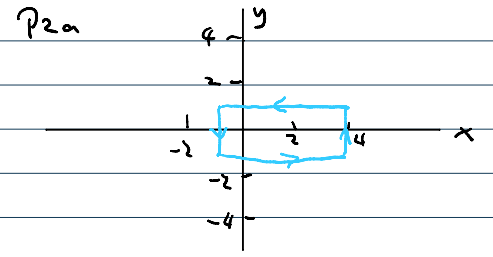
\includegraphics[width=3in]{p3a.png}
                    \end{center}
              \item [(b)] Evaluate $\mathlarger{\int_\gamma\frac{e^z\sin z}{z-2i}dz}$.\\
                    \textbf{Answer}: Since $2i$ is outside the path $\gamma$, we have $\mathlarger{\int_\gamma\frac{e^z\sin z}{z-2i}dz}=0$ by Cauchy's integral theorem.
              \item [(c)] Find $A,B\in\mathbb{C}$ such that $\dfrac{1}{z(z-\pi)}=\dfrac{A}{z}+\dfrac{B}{z-\pi}$.\\
                    \textbf{Answer}: From $\dfrac{1}{z(z-\pi)}=\dfrac{A}{z}+\dfrac{B}{z-\pi}$, we have $1=A(z-\pi)+Bz$. Then at $z=0$ we have $1=-A\pi\implies A=-\pi^{-1}$. Simiarly, at $z=\pi$ we have $1=B\pi\implies B=\pi^{-1}$.
              \item [(d)] Evaluate $\mathlarger{\int_\gamma\frac{e^z\sin z}{z(z-\pi)}dz}$.\\
                    \textbf{Answer}: Using part (c) we have $\mathlarger{\int_\gamma\frac{e^z\sin z}{z(z-\pi)}dz=\int_\gamma\frac{e^z\sin z}{-\pi z}+\int_\gamma\frac{e^z\sin z}{\pi(z-\pi)}}$. We can now evaluate the two integrals separately. Let $f(z)=e^z\sin z$, $a=0$ and $b=\pi$. Then by Cauchy's integral formula we have $\mathlarger{\int_\gamma\frac{e^z\sin z}{-\pi z}=2\pi if(a)}=0$ and $\mathlarger{\int_\gamma\frac{e^z\sin z}{\pi(z-\pi)}=2\pi if(b)=0}$. Therefore $\mathlarger{\int_\gamma\frac{e^z\sin z}{z(z-\pi)}dz}=0$.
          \end{itemize}
    \item [P3] Let $\gamma$ be a simple closed path in $\mathbb{C}$ and suppose that $f(z)$ and $g(z)$ are analytic on and inside $\gamma$. Show that if $f(z)=g(z)$ for all $z$ on $\gamma$, then $f(z)=g(z)$ for all $z$ inside $\gamma$ as well.\\
          \textbf{Answer}: 
    \item [P4] Consider the entire function $f:\mathbb{C}\rightarrow\mathbb{C}$ given by $f(z)=\cos(z)$, which is not constant. Why doesn't this contradict Liouville's Theorem?\\
          \textbf{Answer}: Let $z=x+iy$, then $\cos z=\cos(x+iy)=\cos(x)\cos(iy)-\sin(x)\sin(iy)=\cos(x)\cosh(y)-\sin(x)\sinh(y)$. Since $\cosh(y)$ and $\sinh(y)$ are not bounded, neither is $\cos(z)$. Therefore Liouville's Theorem does not apply.
    \item [P5] Let $f:\mathbb{C}\rightarrow\mathbb{C}$ be entire with $\Re(f(z))\leq 0$ for $z\in\mathbb{C}$.
          \begin{itemize}
              \item [(a)] Show that $e^{f(z)}=\alpha$ for some constant $\alpha\in\mathbb{C}$.\\
                    \textbf{Answer}: Let $u=\Re f(z)$ and $v=\Im f(z)$. Then $\abs*{h(z)}=\abs*{e^{u+iv}}=\abs*{e^u\cdot e^{iv}}=e^u$. Since $u=\Re f(z)\leq 0$, we have $\abs*{h(z)}\leq 0$. Therefore $h(z)$ is entire and bounded, then by Liouville's Theorem it is constant.
              \item [(b)] Show that $f(z)=\beta$ for some constant $\beta\in\mathbb{C}$.\\
                    \textbf{Answer}: Since $e^{f(z)}=\alpha$, we can differentiate both sides which gives us $f'(z)e^{f(z)}=0$. Since $e^{f(z)}$ is always nonzero, we must have $f'(z)=0$. Therefore $f(z)$ is constant.
          \end{itemize}
    \item [P6] Let $f:\mathbb{C}\rightarrow\mathbb{C}$ be entire with $\abs*{f(z)}\leq e^{\Re(z)}$ for $z\in\mathbb{C}$. Show that either
          \begin{itemize}
              \item $f(z)=0$ for every $z\in\mathbb{C}$, or
              \item $f(z)\neq 0$ for any $z\in\mathbb{C}$.
          \end{itemize}
\end{itemize}
\end{document}